\section{System Description}
\def\hyp{\mathbf{w}}
\def\boldxi{\mbox{\boldmath$\xi$}}
\def\smallboldxi{\mbox{\boldmath\scriptsize{$\xi$}}}

The challenge as described was clearly separated into two phases. First, we needed to classify the given audio samples into normal or pathological. Then, the pathological samples were to be classified into one of three kinds: vocal palsy, phonotrauma or neoplasm. Upon an initial inspection and analysis of the data, we observed that vocal palsy seemed the easiest to tell apart from normal by listening to the samples. Therefore, we decided upon a pipeline based approach (Figure~\ref{fig:pipeline}). In the pipeline, after preprocessing, we first check if a new sample is normal or not. If a sample is classified as abnormal, it is sent to the second stage, where we decide if it is a sample corresponding to vocal palsy. If this stage returns negative, we proceed to the final stage where the sample is assigned a label corresponding to either phonotrauma or neoplasm. An advantage of this approach instead of a simple multiclass approach is that, by eliminating many samples for consideration by the later stages of the pipeline, we may hope to improve accuracy over classifying everything at once. On the other hand, this approach leaves the most ``confusing" examples for the last classifier, and since we do not have the option of returning an ``I don't know" label, it may be that our phonotrauma vs neoplasm classifier could have a lower accuracy.

The next consideration was the algorithm to use as a classifier in each stage. Recent machine learning systems and competitions~\cite{b20}\cite{b21} have shown that ensemble approaches are often the best at solving complex problems. This is because typically, a diverse ensemble of classifiers can have elements that each focus on a different aspect of the problem so that when results are combined, the entire system does well. We also chose to follow this principle in designing our classifiers. 

The next question to answer was how to design our ensemble. Rather than going with an off-the-shelf approach, we chose to build an ensemble that was customized to the problem. In particular, we decided to select our ensemble classifiers from three different paradigms: supervised, semi-supervised and multiple-instance learning. The choice of supervised learners was obvious since this task was set up as a batch supervised problem. However, the challenge organizers also provided an unlabeled test set, which was twice the size of the training set. We realized that this could be used as additional information during training. This was especially the case since (as we describe later) we found that doing well on the training set  using cross validation did not guarantee good results on the test set. Therefore we added a semi-supervised component~\cite{b18} which could use the unlabeled test data during learning. Finally, the task as described can also be formulated as a multiple-instance (MI) problem. In MI learning, an example is described by a {\em set} (called a bag) of feature vectors. If an example is labeled positive, at least one instance in the bag is positive; if it is negative, all instances are negative. The task is to learn a bag or instance classifier from such data. In the given task, suppose we partition the given audio samples into windows of some time intervals. Then, we argue that if a voice sample exhibits vocal palsy, or phonotrauma, or neoplasm, {\em there must be at least one window} which contains a signal of that abnormality. Conversely, if a sample is normal, no window contains any abnormality. Therefore this maps well onto the MI learning task. This approach may perform better than analyzing the entire sample because it is possible for most of a sample to be ``normal" even though the patient has a disease. ``Focusing" on a specific fragment of a sample may therefore be better than considering the sample as a whole.

We instantiated the three paradigms as follows.  For supervised learning we used a support vector machine~\cite{b12} (SVM). SVMs are well-known classification algorithms that have demonstrated excellent performance in many practical applications. They were also evaluated in prior work on this task~\cite{b9}. An SVM learns a linear classifier which maximizes the margin by solving the quadratic program (QP): $\underset{\hyp,b,\smallboldxi}{\min}\tfrac{1}{2}\left\lVert  \hyp\right\rVert^2 + C\sum_{i}\xi_i$, such that $y_i\left(\left<\hyp,\phi(x_i)\right> + b\right) \ge 1 - \xi_i$ and $\boldxi \ge 0$. The slack variables $\boldxi=\{\xi_i\}$ allow for
some misclassification of points, and the objective function seeks to minimize
this error on the training data. $C$ is a parameter that trades off  error and
regularization. The dual form of the QP shows that the
separator $\mathbf{w}, b$ can written as a dot product $\langle
\phi(x),\phi(y)\rangle$, so we can use a kernel function $k(x,y)$ to
implicitly represent the feature space $\phi$. We use linear and radial basis function (RBF) kernels in our system. The linear kernel is simply $k(x_i,x_j)= x_i\cdot x_j$ while the RBF kernel is defined by $k(x_i,x_j) = exp(-\gamma||x_i - x_j ||^2)$\cite{b12}.

For semi-supervised learning, we used two approaches: label propagation~\cite{b13} and a transductive SVM~\cite{b22}. Label propagation (LP) assumes a set of labeled and unlabeled points that are arranged as a graph. Edges on the graph are weighted by similarity. LP computes a real-valued function $f: V\rightarrow R$ on the vertices of the graph that minimizes an energy function $E(f)=\sum_{i,j}w_{ij}(f(i)-f(j))^2$, where $w_{ij}$ is the weight on the edge $(i,j)$. The solution can be obtained in closed form and produces a labeling of all unlabeled points in the set of examples. Transductive SVMs extend the basic SVM QP by adding constraints for all unlabeled points, while leaving their labels unknown to be set by the optimizer: $\underset{\hyp,b,\smallboldxi,y_u}{\min}\tfrac{1}{2}\left\lVert  \hyp\right\rVert^2 + C\sum_{i}\xi_i+ \hat{C}\sum_{u}\xi_u$, such that $y_i\left(\left<\hyp,\phi(x_i)\right> + b\right) \ge 1 - \xi_i$, $y_u\left(\left<\hyp,\phi(x_u)\right> + b\right) \ge 1 - \xi_u$, $y_u \in \{-1,+1\}$, $\boldxi \ge 0$. Here the variables indexed by $u$ correspond to the unlabeled set. This is a mixed integer programming problem which is NP-hard to solve in the worst case. However, heuristic approaches exist that have been shown to perform well~\cite{b22}.

For multiple-instance learning, we use multiple-instance logistic regression (MI/LR)~\cite{b10}. This algorithm estimates the probability $\Pr(y_i=1|B_i)$ for a bag $B_i$ from the instances $\{B_{i1},B_{i2},... ,B_{in}\}$ in it. To do this it uses logistic regression to estimate conditional probabilities for each instance,
and softmax to combine these to obtain the conditional
probabilities for each bag:
\begin{eqnarray}
S_{ij}=\Pr(y_{ij}=1|B_{ij})=\frac{1}{1+e^{-({\bf w}\cdot
    B_{ij}+b)}} \nonumber\\
\Pr(y_i=1|B_i)=\mbox{softmax}_\alpha(S_{i1},\ldots,S_{in}) \nonumber
\end{eqnarray}
Note that here, the softmax function encodes the MI assumption that labels a bag positive if at least one instance in it is positive.

To combine the output of these ensembles, we use the following strategy. Initial testing showed that MI/LR had a very high cross-validated area under the ROC graph (AUC) score, sometimes exceeding $0.9$. Therefore we combine the outputs of the predictors as follows: a sample is labeled positive if MI/LR's conditional probability exceeds $0.85$, and negative if the conditional probability is below $0.15$. If the conditional probability lies between these values, or if MI/LR was not in the ensemble, then we return a majority vote of the elements of the ensemble.

We also considered stratifying our models based on gender. Some prior work~\cite{b9} suggests that features may have different distributions in men and women and so there may be value in training separate models. However, we had limited training data and further subdividing it to train gender-specific models did not seem feasible.

\subsection{Data Preprocessing, Implementation and Validation}
A check on the data showed that there was a period of silence at the beginning of most audio files. We removed these parts by calculating the average loudness of each audio file, and removing the prefix of the file that was below  30\% of the average loudness. No other preprocessing was performed on the given data.

Most of our algorithms and features were implemented in Python. We used the libraries Scikit-learn~\cite{b17}, pyAudioAnalysis~\cite{b6} and TSVM~\cite{b23} in our implementation. The MI/LR implementation was done in Java.

Our internal experimentation on the training sets with the supervised and multiple-instance algorithms were performed using 5-fold cross validation. We used these experiments to pick the supervised algorithms to use in our ensemble. We also tried using other approaches such as decision trees and random forests, but they did not perform well on our data.

The SVM classifiers have hyperparameters that need to be tuned. Since the size of training set is getting smaller and smaller as we propagate through the pipeline, in order to tune hyperparameters for all three ensembles, we use the same hyperparameter value obtained in the first ensemble (normal/pathological). Tuning is done through internal cross validation for the hyperparameters $C$ and $\gamma$ independently. The tuned values are 10 for C, and 0.01 for $\gamma$. We also modify the class weight with respect to the proportion of class in the objective function of the SVM in order to correct for class imbalance, since (for example) in the initial task there are only 50 normal samples and 150 pathological cases. This class imbalance parameter is also tuned via the same procedure. 

% \subsection{Validation Method:}
% Before mentioning detailed structure and algorithm we have attempted, I want to point out that we measure accuracy using stratified 10-fold cross validation(CV). Any classifier's accuracy is the weighted average accuracy of numbers we get from 10 folds.  \\
% \indent However, for transductive learning algorithm such as Transductive Support Vector Machine or Label Propagation, we could not do cross validation since there is no validation set for transductive learning. Accuracy we have on those algorithms is the accuracy on whole training set, in other word, the rate of convergence. 
% % \subsection{Attempted Algorithms:}
% Tree-Based Algorithms:
% \begin{itemize}
	% \item Decision Tree:\\
	% Utilizing tree structures, decision tree algorithm calculates entropy of each feature and splits node based on the rank of features with respect to their entropies. Probably due to the fact that different classes are representative in different features and skewed class distribution, a single decision tree could not solve this learning problem and we only get 62\% accuracy on CV.\\
	% \item Random Forest:\\
	% Instead of having a single tree structure, Random Forest fits a number of decision tree classifiers on various sub-samples of the dataset.\cite{b7} Using Random Forest classifier, we get 89\% accuracy on CV. But even with such high accuracy, Random Forest performs poorly on test set according to the feedback from oracle. We analyze that the differences on performance between training set and testing set probably result from skewed data distribution and over-fitting. \\
% \end{itemize}

% \indent Based on cross validation results on experiments we have done, it seems like tree-based algorithm generally is inappropriate for this learning task. \\

% Support Vector Machines(SVMs):\\
% \begin{itemize}
	% \item Linear SVM:\\
	% Based on the features' distribution of each training example, SVM differentiates classes by building a hyperplane that maximizes the margin between classes. And for Linear SVM, the decision boundary is a linear function. The kernel of Linear SVM is simply the hyperplane function $K(x_i,x_j) = \phi(x_i)*\phi(x_j) = (x_i*x_j)^2$, and in order to maximize the margin between plus-plane and minus-plane to get best generalization, SVM minimized the norm of parameter $w$\cite{b12}. After tuning loss penalty and class weight, we get 89\% accuracy on CV and a relatively reasonable classification on test set according to the feedback from oracle.\\
	% \item SVM with Radial Basis Function kernel(SVM-RBF):\\
	% Pretty similar to Linear SVM, SVM-RBF differs by the non-linear kernel function. The SVM-RBF formulation differs from Linear SVM by having an non-linear kernel function, which could be represented as $K(x_i,x_j) = exp(-\gamma||x_i - x_j ||^2)$\cite{b12}. After having a reasonable result from Linear SVM, we were excited on trying SVM-RBF(with tuned loss penalty and gamma). It ends up having 89\% on CV and similar test set performance. However in the late phase, we discarded SVM-RBF because with the number of features we have, it is possible that a non-linear kernel function over-fits. \\
% \end{itemize}

% Transductive Learning Algorithms:\newline\\
% \indent Noticing that size of test set is twice size of training set, in order to get better generalization, we want to utilize test set and attempted several transductive learning algorithms. \\
% \begin{itemize}
	% \item Label Propagation:\\
	% Identifying the test example's closest training set neighbor, Label Propagation assigns the same label that neighbor has to the test example. The edge between any two examples i and j, is weighted to be so that the closer the nodes are in local Euclidean distance, the larger the weight $w_{ij}$, the weight is controlled by a parameter $\theta$ :  $w_{ij} = exp (\frac{(d_{ij}^2)}{\theta^2}) = exp (-\frac{\sum_{d = 1}^{D} (x_{id} - x_{jd})^2}{\theta^2} )$. \cite{b13}Without CV on this algorithm, we compare the number of assigned labels of each class to that from SVMs. From Label Propagation, we get 69 Normals, 107 Vocal Palsys and 171 Phonotraumas. From Linear SVM, we get 65 Normals, 79 Vocal Palsys and 167 Phonotraumas.\\
	% \item Transductive Support Vector Machine(TSVM):\\
	% This is a SVM-RBF based classifier with test set regulating the range of how far away the hyperplane can extends. The kernel function of SVM-RBF is represented as $K(x_i,x_j) = exp(-\frac{||x_i - x_j ||^2}{2\gamma^2})$\cite{b14}. Although in test set, TSVM overcalls a great number of Normal, it could give us a board view of all 'Normal-ish' examples, and later on we could limit our focus on this specific set of Normals. \\
% \end{itemize}

% Multiple Instance Learning Regression(MILR):\\
% \begin{itemize}
	% \item 
	% Instead of receiving a set of instances which are individually labeled, the learner receives a set of labeled bags, each containing many instances. In the simple case of multiple-instance binary classification, a bag may be labeled negative if all the instances in it are negative. On the other hand, a bag is labeled positive if there is at least one instance in it which is positive. \cite{b10} Although MILR undercalls Normal, having super high Area under ROC Curve(AUC) 0.92, MILR could work as an oracle and we only focus on test examples labeled with confidence higher than 85\%.\\
% \end{itemize}
% \subsection{Final Architecture Overview:}
	% Our whole model-building infrastructure is based on scikit-learn\cite{b7}\cite{b8}. \\
	% \indent We tried Support Vector Machine, Boosting, Random Forest, Extratrees, Multiple Instance Learning, Label Propagation. After few experiments, it seemed like tree algorithms performed poorly on this task and we finalized our focus on SVM, Label Propagation, SVM-RBF and MILR with pipeline. Any single classifier undercalled Normal and Neoplasm patients, which we think is resulted from different class distributions between training and testing set. \\
% \indent So, we converted this relatively complex learning task into three less complicated tasks: Normal vs. Pathological, Vocal vs. Rest of Diseases, and Phonotrauma vs. Neoplasm, with each learning task having ensemble consisted of 4 classifiers.[Fig. 1] The reason why we design the pipeline this way is based on the difficulty of classification according to our perception. (From easiest Normal vs. Pathological to hardest Phonotrauma vs. Neoplasm)\\

	\begin{figure}[!htbp]
		\begin{center}
			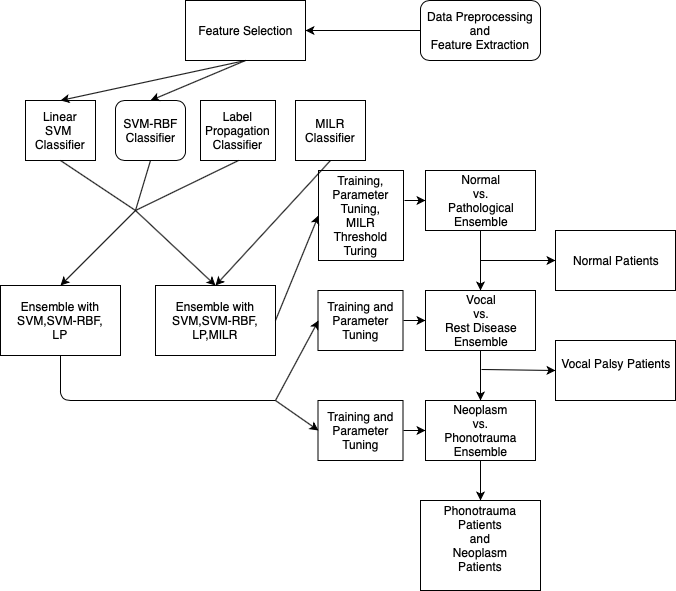
\includegraphics[scale=0.35]{Diagram_3.png}
		\end{center}
		\caption{The Process of Classifying, including classifier training, ensemble structures and pipeline implementation}
		\label{fig:pipeline}
	\end{figure}

% \subsection{Feature Selection:}
% Due to the fact that the size of our training set is relatively small, in case of over-fitting, for each classifier we select 50\% best features, with respect to entropy, according to Renyi's feature selection.\cite{b14} However, it seems like feature selection jeopardizes the performance of transductive learning. So we only utilize feature selection on SVM and SVM-RBF.

% \subsection{Hyper Parameter Tuning:}
% Since the size of training set is getting smaller and smaller as we propagate through the pipeline, in order to get trustworthy accuracy to tune parameter for SVC, for all three ensembles, we use the same parameter tuned in the first ensemble. The process is pretty straightforward; we simply set up two loops, one of which for C and one of which for gamma. The tuned parameters are 10 for C, and 0.01 for gamma. Also due to the skewed distribution in training set, we modify the class weight with respect to the proportion of class. 


